\documentclass[a4paper,12pt]{article}

\usepackage{prettylatex}
\usepackage{titlepage}
\usepackage{boiboites}
\usepackage{pgfplots}

\top{Université de Technologie de Belfort-Montbéliard}{}
\title{Cours d'IN41}{Chapitre 2 -- Analyse des signaux périodiques}
\author{}
\date{Semestre de printemps 2016}

\newboxedtheorem[boxcolor=orange, background={rgb:white,20;green,2;black,1}, titlebackground={rgb:white,15;green,5;black,3},
titleboxcolor = black]{defi}{Définition}{cmpDefi}

\begin{document}

\maketitlepage

\tableofcontents
\pagebreak

\section{Représentation d'un signal}

Un signal ($s(t) = A \cos(2\pi f_{0}t + \alpha)$) peut être représenté dans un espace à 3 dimensions :
\begin{itemize}
    \item projection sur l'axe du temps $\implies$ une sinusoïde continue
    \item projection sur l'axe des fréquences $\implies$ une raie située en $f = f_{0}$ et de hauteur $A$
\end{itemize}

\section{Les séries de Fourier}

\begin{defi}[Série de Fourier]
    Toute fonction $T$-périodique $s$ peut être décomposée en une somme infinie de fonctions sinusoïdales dont les fréquences sont des multiples de la fréquence fondamentale $f_{0} = \dfrac{1}{T}$.
    \[ s(t) = \dfrac{a_{0}}{2} + \sum_{k=1}^{+\infty} a_{k} \cos(2\pi k f_{0} t) + b_{k} \sin(2\pi k f_{0} t) \]
    \[ \text{avec } \begin{cases}
        \dfrac{a_{0}}{2} & \text{ : valeur moyenne ou composante continue} \\
        a_{k} = \frac{2}{T} \int_ {-T/2}^{T/2} s(t) \cos(2\pi f_{0} kt) \mathrm{d}t & \text{ : coefficient de Fourier en cosinus} \\
        b_{k} = \frac{2}{T} \int_ {-T/2}^{T/2} s(t) \sin(2\pi f_{0} kt) \mathrm{d}t & \text{ : coefficient de Fourier en sinus}
    \end{cases} \]
\end{defi}

\paragraph{Harmonique de rang k du signal :}
\[ h_{k}(t) = a_{k} \cos(2\pi kf_{0}t) + b_{k} \sin(2\pi kf_{0}t) \]

\subsection{Séries de Fourier en cosinus}

En prenant en compte la relation :
\[ A \cos(x) + B \sin(x) = \sqrt{A^2 + B^2} \times \cos(x + \arctan(\dfrac{-B}{A})) \]
le développement en séries de Fourier peut s'écrire :
\[ s(t) = A_0 + \sum_{k=1}^{+\infty} A_k \cos(2\pi kf_0 t + \alpha_k) \]

La représentation spectrale qui lui est associée porte le nom de spectre unilatéral.

\subsection{Séries de Fourier complexes}

Rappel de la relation d'Euler :
\[ \cos(\theta) = \dfrac{e^{i\theta} + e^{-i\theta}}{2} \text{ et } \sin(\theta) = \dfrac{e^{i\theta} - e^{-i\theta}}{2i} \]

On montre que la série de Fourier peut être transformée en une série complexe :
\[ s(t) = \sum_{k = -\infty}^{+\infty} X(ik) e^{i2\pi kf_0 t} \]
avec $X(ik)$ le coefficient complexe de la série de Fourier :
\[ X(ik) = \dfrac{1}{T} \int_{-T/2}^{T/2} s(t) e^{-i2\pi kf_0 t} \mathrm{d}t \]

La représentation spectrale qui lui est associée porte le nom de spectre bilatéral.
\[ X(ik) = \dfrac{a_k - ib_k}{2} \text{ et } X(-ik) = \dfrac{a_k + ib_k}{2} \]
\[ a_k = X(ik) + X(-ik) \text{ et } b_k = i[X(ik) - X(-ik)] \]
\[ \arg(X(ik)) = -arg(X(-ik)) = \alpha_k \]

\paragraph{Dans le cas des spectres bilatéraux :}
\[ ||X(ik)|| = ||X(-ik)|| = \dfrac{A_k}{2} \text{ avec } k\neq0 \]
\[ ||X(0)|| = A_0 \]
\[ ||X(ik)|| = ||\dfrac{a_k - ib_k}{2}|| = \dfrac{\sqrt{a^{2}_{k} + b^{2}_{k}}}{2} = \dfrac{A_k}{2} \]
\[ \arg(X(ik)) = \arctan(\dfrac{-b_k}{a_k}) = \alpha_k = -\arctan(\dfrac{b_k}{a_k}) = -arg(X(ik)) \]

\subsection{Quelques propriétés des séries de Fourier :}
\[ X(ik) = \dfrac{A_k}{2} e^{i\alpha_k} \]
\[ X(-ik) = \dfrac{A_k}{2} e^{-i\alpha_k} \]

\paragraph{Signal pair (s(t) = s(-t)) :}
\[ a_k = \dfrac{4}{T} \int_{0}^{T/2} s(t) \cos(2\pi kf_0 t) \mathrm{d}t \text{ et } b_k = 0 \]

\paragraph{Signal pair (s(t) = s(-t)) :}
\[ a_k = 0 \text{ et } b_k = \dfrac{4}{T} \int_{0}^{T/2} s(t) \sin(2\pi kf_0 t) \mathrm{d}t \]

\textbf{Exemple :}

Soit le signal $s$ : $s(t) =
\begin{cases}
    \frac{\pi}{4} & \text{ si } t \in ] 2n\pi ; (2n+1)\pi [ \\
    \frac{-\pi}{4} & \text{ sinon}
\end{cases}$

$s$ est impair $\implies a_k = 0 \text{ et } b_k = \dfrac{-1}{2k} [cos(kt)]_{0}^{\pi} = \dfrac{1}{2k} \times -cos(kt+1)$

\subsection{Suites d'impulsions}

\subsubsection{Suites d'impulsions rectangulaires}

Impulsions rectangulaires de largeur $2\Delta t$ et de période $T$ :
\[ X(ik) = \dfrac{A\Delta t}{T} \underbrace{\dfrac{\sin(k\pi f_0 \Delta t)}{k\pi f_0 \Delta t}}_{=\mathrm{sinc}(k\pi f_0 \Delta t)} \]

\begin{figure}[!htbp]
	\centering
    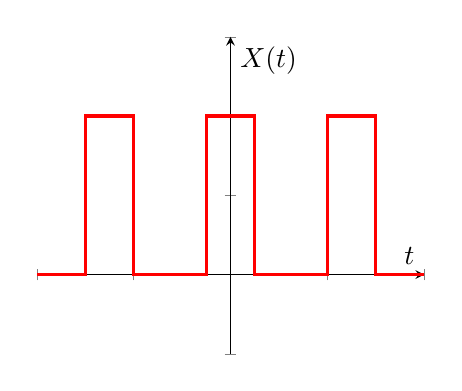
\begin{tikzpicture}
    	\begin{axis}[
            small, axis x line=middle, axis y line=center, xlabel=$t$, ylabel=$X(t)$, xmin=-4, xmax=4, ymin=-0.5, ymax=1.5,
            xticklabels={,,}, % to hide the numbers on the x axis
            yticklabels={,,} % to hide the numbers on the y axis
            ]
            \addplot+[very thick, red, mark=none, const plot] coordinates {(-4,0) (-3,1) (-2,0) (-0.5,1) (0.5,0) (2,1) (3,0) (4,0)};
    	\end{axis}
    \end{tikzpicture}
	\caption{Représentation de la suite d'impulsions rectangulaires}
\end{figure}

\subsubsection{Suites d'impulsions triangulaires}

Impulsions triangulaires de largeur $2\Delta t$ et de période $T$ :
\[ X(ik) = \dfrac{A\Delta t}{T} \mathrm{sinc}^2(k\pi f_0 \Delta t) \]

\begin{figure}[!htbp]
	\centering
    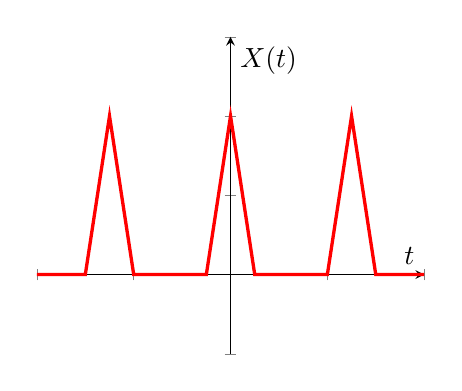
\begin{tikzpicture}
    	\begin{axis}[
            small, axis x line=middle, axis y line=center, xlabel=$t$, ylabel=$X(t)$, xmin=-4, xmax=4, ymin=-0.5, ymax=1.5,
            xticklabels={,,}, % to hide the numbers on the x axis
            yticklabels={,,} % to hide the numbers on the y axis
            ]
            \addplot+[very thick, red, mark=none, sharp plot] coordinates {(-4,0) (-3,0) (-2.5, 1) (-2,0) (-0.5,0) (0,1) (0.5,0) (2,0) (2.5,1) (3,0) (4,0)};
    	\end{axis}
    \end{tikzpicture}
	\caption{Représentation de la suite d'impulsions triangulaires}
\end{figure}

\subsubsection{Suites d'exponentielles décroissantes}

\[ s(t) = \Delta e^{-t/\tau} \text{ avec } \tau \text{ le taux d'amortissement} \]
\[ S(ik) = \dfrac{A}{T} \dfrac{-\tau (e^{-t(\frac{T}{\tau}+i2k\pi f_0 t)})-1}{1+i2\pi kf_0 \tau} \]

 \[ \tau <<< T \implies S(ik) = \dfrac{A\tau}{T} \dfrac{1}{1+i2\pi kf_0 \tau} \]

\subsection{Énergie d'un signal}
\[ E(x) = 1/T \int_{-T/2}^{T/2} s^2(t) \mathrm{d}t \]

\paragraph{Puissance fournie par une harmonique de rang p :}
\[ E_p = \dfrac{1}{T} \int_{-T/2}^{T/2}(a_p \cos(2\pi f_0 pt) + b_p \sin(2\pi f_0 pt)) \mathrm{d}t = \dfrac{a_p^2 + b_p^2}{2} \]

\subsection{Formule de Parseval}

\begin{defi}[Formule de Parseval]
    \[ \dfrac{1}{T} \int_{-T/2}^{T/2} s^2(t) \mathrm{d}t = \dfrac{a_0^2}{4} + \sum_{k=1}^{+\infty} \dfrac{a_k^2 + b_k^2}{2} \]
    \[ \dfrac{1}{T} \int_{-T/2}^{T/2} s^2(t) \mathrm{d}t = A_0^2 + \sum_{k=1}^{+\infty} \dfrac{A_k^2}{2} = \sum_{-\infty}^{+\infty} ||X(ik)||^2 \]
\end{defi}

\subsection{Décalage temporel}

\[ x(t) \longrightarrow y(t) = x(t + t_d) \]
\[ Y(ik) = X(ik) + e^{i2\pi kf_0 t_d} \]
\[ \underbrace{\arg(Y(ik))}_{\beta_k} = \underbrace{\arg(X(ik))}_{\alpha_k} + 2\pi kf_0 t_d \]

\subsection{Modulation d'amplitude}

\[ x(t) = m(t) \times p(t) \]
Si $p(t)$ est sinusoïdale, on peut la remplacer par 2 phaseurs de fréquences $\pm f_p$.
\[ \cos(2\pi kf_pt) = \dfrac{e^{i2\pi kf_pt} + e^{-i2\pi kf_pt}}{2} \]

On montre que :
\[ x(t) = e^{\pm i2\pi f_pt}m(t) \Leftrightarrow X(ik) = M(i(kf_p \pm f_p)) \]

À une multiplication par un phaseur dans le domaine temporel correspond à un décalage dans l'espace de fréquence.

\end{document}
